\question (中国科学技术大学,2004年)在图采用邻接表存储时,求最小生成树的Prim算法的时间复杂度为(
)
\par\fourch{}{}{\textcolor{red}{}}{}
\begin{solution}Prim算法的时间复杂度是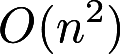
\includegraphics[width=0.43750in,height=0.19792in]{texmath/ead2f65Cdpi7B3507DO28n5E229},与图中边数无关,该算法适合于稠密图。Kruskal算法的时间复杂度是O(eloge),算法的时间复杂度主要取决于边数,较适合于稀疏图。
\end{solution}
\question 下列关于最小生成树的说法中,正确的是( )。 Ⅰ.最小生成树的代价唯一
Ⅱ.所有权值最小的边一定会出现在所有的最小生成树中
Ⅲ.使用普里姆(Prim)算法从不同顶点开始得到的最小生成树一定相同
Ⅳ.使用普里姆算法和克鲁斯卡尔(Kruskal)算法得到的最小生成树总不相同
\par\twoch{\textcolor{red}{仅Ⅰ}}{仅Ⅱ}{仅Ⅰ、Ⅲ}{仅Ⅱ、Ⅳ}
\begin{solution}由一个带权连通图构造的最小生成树可能有多棵,但其代价一定是唯一的,故Ⅰ正确。
权值最小的边可能不唯一,这些不唯一的最小权值边不一定都会出现在所有的最小生成树中,故Ⅱ错误。
当存在多条权值相同的边时,用普里姆(Prim)算法从不同顶点开始得到的最小生成树不一定相同,故Ⅲ错误。
当最小生成树唯一时,无论用哪种算法,得到的最小生成树都是相同的,故Ⅳ错误。
【总结】
在一个具有几个顶点的连通图G中,如果存在子图G'包含G中所有顶点和一部分边,且不形成回路,则称G'为图G的生成树,代价最小生成树则称为最小生成树。当存在相同权值的边时,其最小生成树也可能是不唯一的。
\end{solution}
\question (青岛大学,2004年)对于含有n个顶点e条边的无向连通图,利用Kruskal算法产生最小生成树时,其时间复杂度为(
)
\par\fourch{}{O(n*e)}{O(nlogn)}{\textcolor{red}{O(eloge)}}
\begin{solution}克鲁斯卡尔算法的复杂度主要取决于边数,适合于稀疏图。《高分笔记》当中提到,克鲁斯卡尔算法算法时间主要花在对边的排序函数上,因此最快的算法便是O(eloge)
\end{solution}
